% Objectives Tree Diagram for SNC Subsystem
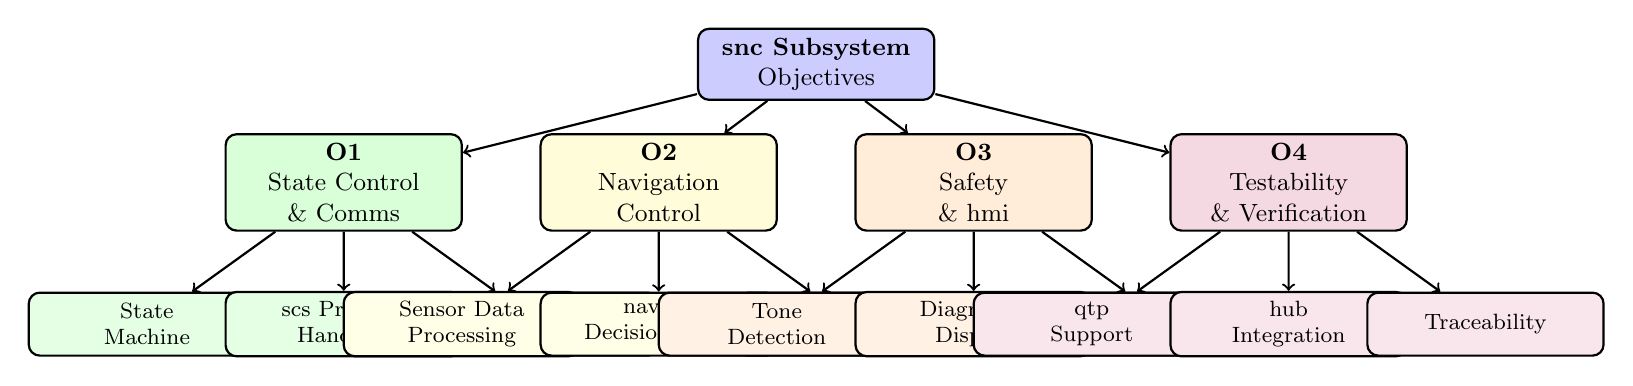
\begin{tikzpicture}[
  level 1/.style={sibling distance=4cm, level distance=1.5cm},
  level 2/.style={sibling distance=2.5cm, level distance=1.8cm},
  every node/.style={
    rectangle,
    rounded corners,
    draw=black,
    thick,
    minimum width=3cm,
    minimum height=0.8cm,
    align=center,
    font=\small
  },
  edge from parent/.style={draw, thick, ->}
]

% Root node
\node[fill=blue!20] {\textbf{\gls{snc} Subsystem}\\Objectives}
  child {
    node[fill=green!15] {\textbf{O1}\\State Control\\\& Comms}
    child {node[fill=green!10, font=\footnotesize] {State\\Machine}}
    child {node[fill=green!10, font=\footnotesize] {\gls{scs} Protocol\\Handling}}
    child {node[fill=green!10, font=\footnotesize] {Transition\\Guards}}
  }
  child {
    node[fill=yellow!15] {\textbf{O2}\\Navigation\\Control}
    child {node[fill=yellow!10, font=\footnotesize] {Sensor Data\\Processing}}
    child {node[fill=yellow!10, font=\footnotesize] {\gls{navcon}\\Decision Logic}}
    child {node[fill=yellow!10, font=\footnotesize] {Motion\\Commands}}
  }
  child {
    node[fill=orange!15] {\textbf{O3}\\Safety\\\& \gls{hmi}}
    child {node[fill=orange!10, font=\footnotesize] {Tone\\Detection}}
    child {node[fill=orange!10, font=\footnotesize] {Diagnostic\\Display}}
    child {node[fill=orange!10, font=\footnotesize] {\gls{pec}\\Compliance}}
  }
  child {
    node[fill=purple!15] {\textbf{O4}\\Testability\\\& Verification}
    child {node[fill=purple!10, font=\footnotesize] {\gls{qtp}\\Support}}
    child {node[fill=purple!10, font=\footnotesize] {\gls{hub}\\Integration}}
    child {node[fill=purple!10, font=\footnotesize] {Traceability}}
  };

\end{tikzpicture}
